\documentclass[10pt]{article}
\usepackage[brazil]{babel} % ABRASILEIRAR O TRABALHO
\usepackage[utf8]{inputenc} % PERMITE USAR DIGITAÇÃO COMO NO WORD
\usepackage{amsfonts}
\usepackage{amssymb,amscd,latexsym}
\usepackage{amsmath}
\usepackage{amsthm}
\usepackage{epsfig}
\usepackage{color}
\usepackage{multicol}
\usepackage{soul}
\usepackage{cancel}
\usepackage[top=3cm,bottom=2cm, left=3cm,right=2cm]{geometry}
\usepackage{tikz}
\usepackage{pgfplots}
\usepackage{enumitem}
\usepackage{dsfont}
\usepackage{titling}
\usepackage{gensymb}
\usepackage{pifont}
\usepackage{graphicx}
\usepackage{color}
\usepackage{wrapfig}
\usepackage{stackrel}
\usepackage{cancel}
\usepackage{mathptmx} %Pacote da fonte tipo Times New Roman
\usepackage{animate}

\usepackage{subcaption}
\usepackage{accents}
\usepackage{stackrel}
\usepackage{icomma}
\usepackage{framed}

\usepackage[backend=biber,style=abnt]{biblatex}  
\bibliography{biblio} %Definição do arquivo de bibliografia tipo BibTeX

\graphicspath{{img/}} %Indicação da pasta de imagens
\usetikzlibrary{arrows,intersections}
\pgfplotsset{width=7cm,compat=1.12}

%%%%%%%%%%%%%%%%%%%%%%%%%%%%%%%%%%%%%%%%%%%%%%%
%Definições de estilos de teoremas, proposições
\theoremstyle{plain}
\newtheorem{teor}{Teorema}[section]
\newtheorem{prop}[teor]{Proposição}
\newtheorem{lema}[teor]{Lema}
\newtheorem{cor}[teor]{Corolário}
\newtheorem*{afirmacao}{Afirma\c c\~ao}
\theoremstyle{remark}
\newtheorem*{obs}{Observação}
\theoremstyle{definition}
\newtheorem{definition}[teor]{Definição}
\newtheorem{exe}[teor]{Exemplo}
\newtheorem{prob}{Problema}[section]
\renewcommand\qedsymbol{$\blacksquare$}
%%%%%%%%%%%%%%%%%%%%%%%%%%%%%%%%%%%%%%%%%%%%%%%
%Macros

\renewcommand{\csc}{\textrm{\,cosec}\,} %Renomeando cossecante
\renewcommand{\arcsin}{\textrm{\,arcsen}\,} %Renomeando arcoseno
\renewcommand{\sin}{\textrm{\,sen}\,} %Renomeando seno
\renewcommand{\tan}{\textrm{\,tg}\,} %Renomeando tangente
\newcommand{\cotan}{\textrm{\,cotg}\,} %Renomeando cotangente
\newcommand{\var}{\textrm{Var}\,} %Variância
\newcommand{\vet}[3]{\overrightarrow{#1}=(#2,#3)} %Vetor 2d
\newcommand{\vett}[4]{\overrightarrow{#1}=(#2,#3,#4)} %Vetor 3D
\newcommand{\sva}[2]{#1_{1},#1_{2},\ldots,#1_{#2}} %Sequência de variáveis aleatórias com letra igual ao primeiro parâmetro e tamanho igual ao segundo
\newcommand{\resp}[1]{\textcolor{red}{R: #1}} %Usado em listas para resposta
%%%%%%%%%%%%%%%%%%%%%%%%%%%%%%%%%%%%%%%%%%%%%%%

\title{Valores P}
\author{Augusto César F. de Miranda Oliveira}
\date{\today}
\makeatletter
%%%%%%%%%%%%%%%%%%%%%%%%%%%%%%%%%%%%%%%%%%%%%%%
%Fim do preâmbulo

\begin{document}
%Início da página de título
\begin{titlepage}
\begin{center}

\includegraphics[height=2.5cm]{logo.png} \\ % inclui figura
{\large  UNIVERSIDADE FEDERAL RURAL DE PERNAMBUCO - UFRPE\\
Programa de Pós-Graduação em Biometria e Estatística Aplicada\\
Inferência Estatística\\
Prof. Frank Sinatra\\
}
\vspace{5cm} %Espaço vertical
\Large{\@title}\\ %Título com letra grande
\vspace{5cm}{\@author}\\ %Autor com letra grande
\vspace{5cm}
RECIFE\\
2019
\end{center}
\end{titlepage}
\section{Introdução}
O valor P é derivado da perspectiva de um teste de hipótese, no qual a estatística de um teste é calculada a partir dos resultados de um determinado conjunto de dados sob a hipótese nula ser verdadeira. A distribuição da estatística de teste é utilizada para para obter a menor probabilidade de observar esse resultado (hipótese nula ser verdadeira) ou um resultado mais extremo.

Assim, o valor P é uma medida de evidência contra a hipótese nula. O valor P é baseado na análise de variáveis aleatórias, por isso o mesmo é uma variável aleatória cuja distribuição, para estatísticas de testes contínuas, é conhecida por ser uniforme no intervalo [0,1] sob a hipótese nula. Por esse fato, um ponto de corte para o valor P é utilizado. Geralmente 0.05 é utilizado para controlar as chances de que, para qualquer experimento, o valor P possa ser 0.05 ou menor, sendo a hipótese nula é verdadeira.

Esse conceito, na teoria de Neyman-Pearson de testes de hipóteses, é conhecido como taxa de erro do tipo I, que é uma taxa de erro que determina a região de rejeição e busca controlar a frequência geral de rejeições errôneas da hipótese nula. Outras medidas estatísticas, como intervalos de confiança, podem subsidiar este entendimento, porém não será objeto de estudo deste trabalho.
\section{Valores P}
P-valor ou valor p é outro meio de relatar os resultados de um teste de hipótese, expondo, assim, um valor associado a um tipo de estatística de teste.
\begin{definition}
Um \textit{valor p p}(\textbf{X}) é uma estatística de teste que satisfaz $0 \leq p(\textbf{x}) \leq 1$ para cada ponto amostral \textbf{x}. Pequenos valores de \textit{p}(\textbf{X}) fornecem evidências de que $H_{1}$ é verdadeira. Um valor p é \textit{válido} se, para cada $\theta \in \Theta_{0}$ e cada $0 \leq \alpha \leq 1$,
\begin{equation}
     P_{ \theta } (p(\textbf{X})  \leq  \alpha ) \leq  \alpha.
\end{equation}
Onde,
\begin{itemize}
    \item $P_{ \theta }$ declara a probabilidade de ocorrência de eventos extremos (rejeitar a hipótese nula sabendo que é verdadeira);
    \item $p(\textbf{X})$ é uma estatística de teste sob a população em estudo e
    \item $\alpha$ denota o nível de significância estipulado.
\end{itemize}
Se $p(\textbf{X})$ for um valor válido, é fácil criar um teste de nível $\alpha$ baseado em p(\textbf{X}). O teste que rejeita $H_{0}$, se e somente se, $p(\textbf{X}) \leq \alpha$ é um teste de nível $\alpha$ por causa de (1). Um a vantagem de relatar o resultado de teste por intermédio de um valor p é que cada leitor pode escolher o $\alpha$ que considerar apropriado, e então, pode comparar o $p(\textbf{x})$ relatado a $\alpha$ e saber se esses dados levam à aceitação ou rejeição de $H_0$. Deste modo, um valor p relata os resultados de um teste em uma escala mais contínua, em vez de apenas ``aceitar $H_0$'' ou ``rejeitar $H_0$''.
O meio mais comum para definir um valor p válido é dado pelo Teorema 2.2.
\end{definition}
\begin{teor}
Seja $W(\textbf{X})$ uma estatística de teste, de modo que grande valores de $W$ dão evidências de que $H_1$ é verdadeira. Para cada ponto amostral \textbf{x}, defina
\begin{equation}
    p(\textbf{x}) = \ \sup_{\theta \in \Theta_{0}} \ P_{\theta}(W(\textbf{X}) \geq W(\textbf{x}))
\end{equation}
Então, $p(\textbf{x})$ é um valor p válido.
\end{teor}
\begin{proof}
Fixe $\theta \in \Theta_{0}$. Seja $F_\theta(w)$ denotando a FDA de $-W(\textbf{X})$. Definimos:
\begin{align*}
    p_{ \theta }(\textbf{x}) &=P_{ \theta }(W(\textbf{X}) \geq W(\textbf{x})) \\
    &=P_{\theta}(-W(\textbf{X}) \leq -W(\textbf{x})) \\
    &= F_{ \theta }(-W(\textbf{x})).
\end{align*}
Então, a variável aleatória $p_{\theta}(\textbf{X})$ é igual a $F_{\theta}$(-W(\textbf{X})). Deste modo, de acordo com a \textbf{Transformação Integral de Probabilidade} definida por Magalhães \cite*[p.~150]{marco} como,
\begin{quote}
Seja \textit{X} uma variável com função de distribuição \textit{F}. A transformação de X tal que $Y=F(X)$ é denominada \textit{transformação integral de probabilidade.} \hfill $\square$

Assim, por exemplo, se temos $X \sim Exp(\lambda)$, $F(x)=1-e^{-\lambda x}$ e obtemos a transformação integral $Y=1-e^{-\lambda X}$. Em simulações, o uso da transformação depende da possibilidade de inverter $F$. A inversa tem domínio em [0,1], mas se $F$ tiver saltos ou for em escada, ela não existirá.
A função inversa também, por abuso de notação, pode ser representada por $F^{-1}$.
\end{quote}
Logo, uma distribuição de $p_{\theta}(\textbf{X})$ é estocasticamente maior ou igual a uma distribuição uniforme (0,1). Isto é, para cada $0 \leq \alpha \leq 1$, $P_{ \theta } (p_{ \theta }(\textbf{X})  \leq  \alpha ) \leq  \alpha$. Uma vez que $p(\textbf{x}) = \sup_{\theta' \in \Theta_{0}} p_{\theta'}(\textbf{x}) \geq p_{\theta}(\textbf{x})$ para cada \textbf{x}.
\begin{equation*}
    P_{\theta}(p(\textbf{X} \leq \alpha) \leq P_{\theta}(p_{\theta}(\textbf{X}) \leq \alpha) \leq \alpha).
\end{equation*}
Isto é verdadeiro para cada $\theta \in \Theta_{0}$ e para cada $0 \leq \alpha \leq 1; p(\textbf{X})$ é um valor p válido.
\end{proof}
O cálculo do supremo em (2) pode ser difícil, pois ``[...] alguns conjuntos limitados de números racionais não possuem supremo (ou 
ínfimo). Este fato está ligado à inexistência de raízes quadradas racionais de certos números inteiros, mas é uma dificuldade que vai muito além dessa falta'' \cite[p.~78]{lima2019curso}. Os dois exemplos seguintes ilustram situações comuns nas quais isto não é muito difícil. No primeiro, nenhum supremo é necessário; no segundo, é fácil determinar o valor de $\theta$ em que o supremo ocorre.
\begin{framed}
\begin{exe}[Valor p bilateral da normal]
Sejam $X_{1},...,X_{n}$ uma amostra aleatória de uma população n($\mu, \sigma^{2}$). Considere testar $H_0:\mu=\mu_0$ versus $H_1:\mu \neq \mu_0$. Onde,
\begin{itemize}
    \item $\mu_0$ denota a média amostral do experimento.
    \item $H_0:\mu=\mu_0$ declara que não houve alteração no experimento.
    \item $H_1:\mu \neq \mu_0$ declara que houve alteração no experimento.
\end{itemize}
De acordo acordo com o exercício 8.38 \cite[p.~408]{casella}, o Teste de Razão de Verossimilhança (TRV) rejeita $H_0$ para grandes valores de $W(\textbf{X})=|\overline{x}-\mu_0|/(S/\sqrt{n})$, em que $W(\textbf{X})$ é uma estatística de teste para média. Sabendo-se que, $\sigma$ é desconhecida, por definição temos.
\begin{align}
    W(\textbf{X})=\frac{(\overline{x}-\mu_0)}{(S/\sqrt{n})}, \text{ em que } W(\textbf{X}) \sim T_{n-1}
\end{align}
Calculando (2) para encontrar um valor p válido, temos:
\begin{align}
    p(\textbf{x})&=\sup_{\mu \in \Theta_{0}}P_{\mu}(W(\textbf{X}) \geq W(\textbf{x})) \nonumber \\
    &=P_{\mu}(W(\textbf{X}) \geq W(\textbf{x})) \nonumber \\
    &=2P_{\mu}(T_{n-1} \geq W(\textbf{x})) \nonumber \\
    &=2[1 - P_{\mu}(T_{n-1} < W(\textbf{x}))] \nonumber \\
    &=2\left\{1-F^{-1}_{T_{n-1}}[W(\textbf{x})]\right\}
\end{align}
Em que $F^{-1}_{T_{n-1}}$, é o inverso da Função de Distribuição Acumulada (FDA) \textit{t}-Student com $n-1$ graus de liberdade. Portanto, ao calcular (4), a probabilidade é a mesma para todos os valores de $\mu$, desconsiderando, assim, o cálculo do supremo.

A Figura \ref{fig:bilateral} ilustra o p valor para um teste de hipótese bilateral da normal, onde a ocorrência de valores mais extremos sob a hipótese nula ser verdadeira pode ocorrer nas duas caudas da distribuição.
\begin{minipage}{\textwidth}
\centering
    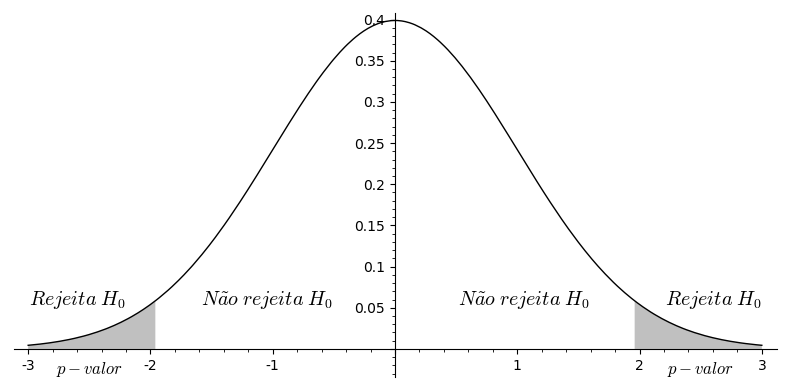
\includegraphics[height=6.5cm]{Bilateral.png}
    \captionof{figure}{Valor p bilateral da normal}
    \label{fig:bilateral}
\end{minipage}
\end{exe}
\end{framed}
\begin{framed}
\begin{exe}[Valor p unilateral da normal]
Mais uma vez, tenha em conta o modelo normal do Exemplo 2.3, mas considere testar $H_{0}:\mu \leq \mu_{0}$ versus $H_{1}: \mu > \mu_{0}$. Onde,
\begin{itemize}
    \item $\mu_0$ é a proporção máxima aceitável de itens com defeito.
    \item $H_{0}:\mu \leq \mu_{0}$ declara que a proporção de itens com defeito é aceitável.
    \item $H_{1}: \mu > \mu_{0}$ declara que a proporção de itens com defeito é inaceitavelmente alta.
\end{itemize}
De acordo com o exercício 8.37 \cite[p.~407]{casella}, o TRV rejeita $H_{0}$ para grandes valores de $W(\textbf{X})=(\overline{X}-\mu_{0})/(S/\sqrt{n})$. O seguinte argumento mostra que, para esta estatística, o supremo em (2) sempre ocorre em um parâmetro $(\mu_{0},\sigma)$, e o valor de $\sigma$ utilizado não faz diferença. Considere qualquer $\mu \leq \mu_{0}$ e qualquer $\sigma$:
\begin{align*}
P_{\mu,\sigma}(W(\textbf{X}) \geq W(\textbf{x})) &=P_{\mu,\sigma}\left(\frac{\overline{x}-\mu_{0}}{S/\sqrt{n}} \geq W(\textbf{x})\right)\\
&=P_{\mu,\sigma}\left(\frac{\overline{x}-\mu_{0} + \mu - \mu}{S/\sqrt{n}} \geq W(\textbf{x})\right)\\
&=P_{\mu,\sigma}\left(\frac{\overline{x}-\mu}{S/\sqrt{n}} + \frac{\mu-\mu_0}{S/\sqrt{n}}\geq W(\textbf{x})\right)\\
&=P_{\mu,\sigma}\left(\frac{\overline{x}-\mu}{S/\sqrt{n}} \geq W(\textbf{x}) - \left( \frac{\mu-\mu_0}{S/\sqrt{n}}\right)\right)\\
&=P_{\mu,\sigma}\left(\frac{\overline{x}-\mu}{S/\sqrt{n}} \geq W(\textbf{x}) + \frac{\mu_{0}-\mu}{S/\sqrt{n}}\right)\\
&=P_{\mu,\sigma}\left(T_{n-1} \geq W(\textbf{x})+\frac{\mu_{0}-\mu}{S/\sqrt{n}}\right)\\
&\leq P(T_{n-1} \geq W(\textbf{x}))
\end{align*}
Aqui, mais uma vez, $T_{n-1}$ tem uma distribuição \textit{t}-Student com $n-1$ graus de liberdade. A desigualdade na última linha é verdadeira porque $\mu_{0} \geq \mu$ e $(\mu_{0}-\mu)/(S/\sqrt{n})$ é uma variável aleatória não negativa. Aqui, o subscrito em \textit{P} é eliminado, porque esta probabilidade não depende de $(\mu,\sigma)$. Além disso,
\begin{center}
    $P(T_{n-1} \geq W(\textbf{x}))=P_{\mu_{0},\sigma}\left(\frac{\overline{X}-\mu_{0}}{S/\sqrt{n}} \geq W(\textbf{x})\right)=P_{\mu_{0},\sigma}(W(\textbf{X}) \geq W(\textbf{x}))$,
\end{center}
e esta probabilidade é uma daquelas consideradas no cálculo do supremo em (2) porque $(\mu_{0},\sigma) \in \Theta_{0}$. Portanto, o valor p de (2) para este teste unilateral $t$ é $p(\textbf{x})=P(T_{n-1} \geq W(\textbf{x}))=P(T_{n-1} \geq (\overline{x}-\mu_{0}/(s/\sqrt{n}))$.
A Figura \ref{fig:unilateral} ilustra o p valor para um teste de hipótese unilateral da normal, onde a ocorrência de valores mais extremos sob a hipótese nula ser verdadeira pode ocorrer apenas na cauda direita da distribuição.\vspace{0.25cm} %Espaço vertical
\begin{minipage}{\textwidth}
\centering
    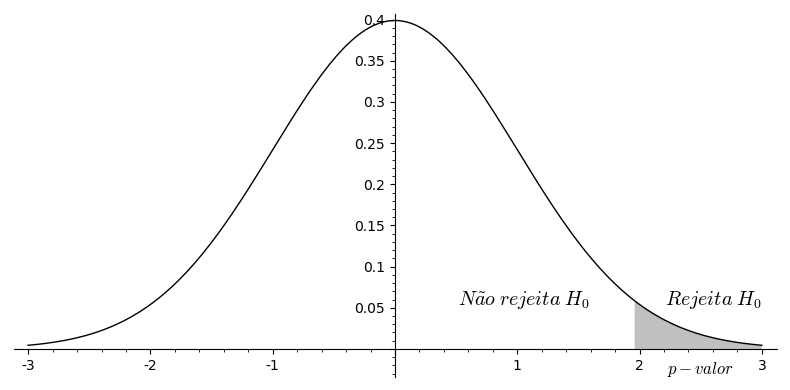
\includegraphics[height=6.5cm]{Unilateral.png}
    \captionof{figure}{Valor p unilateral da normal}
    \label{fig:unilateral}
\end{minipage}
\end{exe}
\end{framed}
Outro método para definir um valor p válido, uma alternativa à utilização de (2), envolve condicionar sobre uma estatística suficiente. Suponha que $S(\textbf{X})$ seja uma estatística suficiente para o modelo $\left\{f(\textbf{x}|\theta): \theta \in \Theta_{0}\right\}$. (Para evitar testes com poder baixo, é importante que S seja suficiente somente para o modelo nulo, não para todo modelo $\left\{f(\textbf{x}|\theta): \theta \in \Theta\right\}$.) Se a hipótese nula for verdadeira, a distribuição condicional de \textbf{X} dado $S=s$ não depende de $\theta$. Mais uma vez, seja $W(\textbf{X})$ denotando uma estatística de teste para a qual grandes valores dão evidência de que $H_{1}$ é verdadeira. Então, para cada ponto amostral \textbf{x} definimos:
\begin{align}
    p(\textbf{x})=P(W(\textbf{X}) \geq W(\textbf{x})|S=S(\textbf{X}))
\end{align}
Argumentando como no Teorema 2.2, mas considerando somente a distribuição única, que é a distribuição condicional de \textbf{X} considerando que $S=s$, vemos que, para qualquer, $0 \leq \alpha \leq 1$, 
\begin{align*}
    P(p(\textbf{X}) \leq \alpha| S=s) \leq \alpha
\end{align*}
Então, para qualquer $\theta \in \Theta_{0}$, temos, incondicionalmente,
\begin{align*}
    P_{\theta}(p(\textbf{X})\leq \alpha)=\sum_{s}P(p(X)\leq\alpha|S=s)P_{\theta}(S=s) \leq \sum_{n}\alpha P_{\theta}(S=s) \leq \alpha
\end{align*}
Deste modo, $p(\textbf{X})$ definido por (5) é um valor p válido. Somas podem ser substituídas pelas integrais para S contínuo, mas este método geralmente é utilizado para S discreto, como no exemplo seguinte. 
\begin{exe}[Teste Exato de Fisher]
 \begin{framed}
 Sejam $S_{1}$ e $S_{2}$ observações independentes, com $S_{1} \sim Binomial(n_1,p_1)$ e $S_{2} \sim Binomial(n_2,p_2)$. Considere testar $H_0: p_1=p_2$ versus $H_1: p_1 > p_2$. De acordo com $H_{0}$, supondo que p denote o valor comum de $p_1=p_2$, a fp conjunta de $(S_1,S_2)$ é
\begin{align*}
    f(s_1,s_2|p)&=\binom{n_1}{n_2}p^{s_1}(1-p)^ {n_1-n_2}\binom{n_2}{p_2}p^{s_2}(1-p)^{n_2-p_2}\\
    &=\binom{n_1}{n_2}\binom{n_2}{s_2}p^{s_1+s_2}(1-p)^{n_1+n_2-(s_1+s_2)}
\end{align*}
Portanto, $S=S_1+S_2$ é uma estatística suficiente, de acordo com $H_0$. Considerando o valor de $S=s$, é razoável utilizar $S_1$ como uma estatística de teste e rejeitar $H_0$ em favor de $H_1$ para grandes valores de $S_1$, porque grandes valores de $S_1$ correspondem a pequenos valores de $S_2=s-S_1$. A distribuição condicional $S_1$ dado $S=s$ é hipergeométrica$(n_1+n_2,n_1,s)$, vejamos:

Sabendo-se que, por definição, a distribuição condicional pode ser reescrita em notação de função de probabilidade da seguinte forma:
\begin{equation*}
    P_{x|y}(x|y)=\frac{P_{x,y}(x,y)}{P_{y}(y)}
\end{equation*}
E, se $X,Y$ são independentes, então $P_{x,y}(x,y)=P_{x}(x)\cdot P_{y}(y)$. Sendo assim, temos:
\begin{align}
    P(S_1=s_1|S_1+S_2=s)&=\frac{P(S_1=s_1,S_1+S_2=s)}{P(S_1+S_2=s)}\nonumber\\
              &=\frac{P(S_1=s_1,S_2=s-S_1)}{P(S_1+S_2=s)}\nonumber\\ 
              &=\frac{P(S_1=s_1,S_2=s-s_1)}{P(S_1+S_2=s)} \nonumber \\
              &=\frac{P(S_1=s_1)P(S_2=s-s_1)}{P(S_1+S_2=s)}
\end{align}
 Onde, 
 \begin{itemize}
     \item $S_1 \sim Binomial(n_1,s_1)=\binom{n_1}{s_1}p^{s_1}(1-p)^{n_1-s_1}$ 
    \item $S_2 \sim Binomial(n_2,s-s_1)=\binom{n_2}{s-s_1}p^{s-s_1}(1-p)^{n_2-(s-s_1)}$
    \item $S_1 + S_2 \sim Binomial(n1+n2,s)=\binom{n_1+n_2}{s}p^{s}(1-p)^{n_1+n_2-s}$
 \end{itemize}
 Retomando a equação (6), temos:
 \begin{align*}
    &=\frac{\binom{n_1}{s_1}p^{s_1}(1-p)^{n_1-s_1}\cdot\binom{n_2}{s-s_1}p^{s-s_1}(1-p)^{n_2-s+s_1}}{\binom{n_1+n_2}{s}p^{s}(1-p)^{n_1+n_2-s}}\\
    &=\frac{\binom{n_1}{s_1}\binom{n_2}{s-s_1}p^{s_1+s-s_1}(1-p)^{n_1-s_1+n_2-s_1+s_1}}{\binom{n_1+n_2}{s}p^{s}(1-p)^{n_1+n_2-s}}\\
    &=\frac{\binom{n_1}{s_1}\binom{n_2}{s-s_1}p^{s}(1-p)^{n_1+n_2-s}}{\binom{n_1+n_2}{s}p^{s}(1-p)^{n_1+n_2-s}}\\
    &=\frac{\binom{n_1}{s_1}\binom{n_2}{s-s_1}}{\binom{n_1+n_2}{s}} \\
    &=\textit{hipergeométrica}(n1+n2,s)
\end{align*}
Assim, o valor p condicional em (5) é
\begin{align*}
p(s_1,s_2)=\sum_{j=s_1}^{min(n_1,s)} f(j|s),
\end{align*}
a soma das probabilidades hipergeométricas. O teste definido por este valor p é chamado de Teste Exato de Fisher. 
 \end{framed}
\end{exe}

%%%o TRV re%%%%%%%%%%%%%%%%%%%%%%%%%%%%%%%%%%%%%%%%%%%%%%
%Página de referências
\newpage 
\printbibliography
\end{document}
